
\documentclass[tikz]{standalone}
\usepackage{lib/basic}
\tikzset{
I/.style={draw=black, fill=green!20, circle, inner 
        sep=0pt, text width=22pt, align=center, line width=1.0pt},
H/.style={draw=black, fill=green!20, circle, inner 
        sep=0pt, text width=22pt, align=center, line width=1.0pt},
NeuralLineLayer/.style={arrows={-latex},draw=black,line width=1.5pt,rounded corners=4pt},
NeuralNetworkTittle/.style={text width=4em, text centered},
NeuralNetworkTittle/.style={text width=4em, text centered},
}
\begin{document}
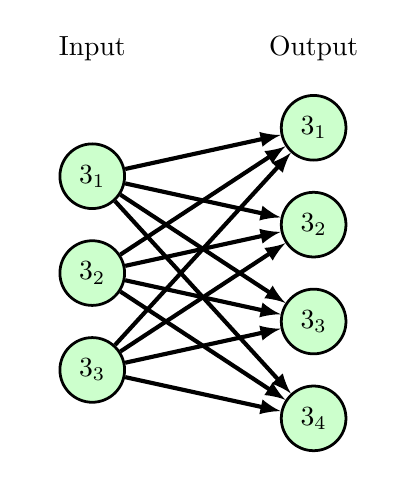
\begin{tikzpicture}[]
	\foreach \y in {1,...,3}
		\node[I,] (I\y) at (0,35pt-\y*35pt) {$3_\y$};
	\foreach \y in {1,...,4}
		\node[H,] (H\y) at (80pt,52.5pt-\y*35pt) {$3_\y$};\foreach \dest in {1,...,3}
        \foreach \source in {1,...,4}
            \draw[NeuralLineLayer] (I\dest) edge (H\source);

	\node[NeuralNetworkTittle, above of=I1]  at (I1 |- H1) {Input};
	\node[NeuralNetworkTittle, above of=H1]  at (H1 |- H1) {Output};
\end{tikzpicture}
\end{document}